\begin{pastexam}[label={px:gw3-098-ds-05}]{關務三等資訊處理 98 年 第五題}
（申論；20 分）

有一檔案其字母集為\{S, T, U, V, W, X, Y, Z\}，字母出現的頻率如下表：
\begin{center}
\small
\begin{tabular}{|c|c|c|c|c|c|c|c|c|}
\hline
字母 & S & T & U & V & W & X & Y & Z \\ \hline
頻率 & 4 & 6 & 10 & 24 & 10 & 2 & 15 & 29 \\ \hline
\end{tabular}
\end{center}
\begin{enumerate}[leftmargin=2.6em, labelsep=0.4em]
\item[㈠] 若以下列不定長度二進位編碼（variable-length binary code）來編碼此檔案，請問每個字母平均用幾個位元表示？（5 分）
\begin{center}
\small
\begin{tabular}{|c|c|c|c|c|c|c|c|c|}
\hline
字母 & S & T & U & V & W & X & Y & Z \\ \hline
編碼 & 00 & 10 & 010 & 011 & 1100 & 1101 & 1110 & 1111 \\ \hline
\end{tabular}
\end{center}
\item[㈡] 霍夫曼碼（Huffman code）是一種與檔案中字母出現頻率有關的不定長度二進位編碼法，檔案經其編碼後，長度是所有
不定長度二進位編碼中最短的。請為此檔案建立其霍夫曼碼，並算出此編碼下每個字母平均用幾個位元表示。（15 分）
\end{enumerate}
\end{pastexam}

\begin{pastsoln}
答案：㈠ $3.46$ 個位元；㈡ $2.65$ 個位元。 頻率總和 $4 + 6 + 10 + 24 + 10 + 2 + 15 + 29 = 100$，「平均」是以頻率加權的
平均：$\sum f_c \cdot \mathit{len}(c) / \sum f_c$。

\textbf{㈠} 這組編碼是前綴碼（沒有一個碼字是另一個的前綴，例如 $00$ 和 $010$、$011$ 第二位就不同）。
\begin{align*}
&\frac{4 \cdot 2 + 6 \cdot 2 + 10 \cdot 3 + 24 \cdot 3 + 10 \cdot 4 + 2 \cdot 4 + 15 \cdot 4 + 29 \cdot 4}{100} \\
&\qquad = \frac{8 + 12 + 30 + 72 + 40 + 8 + 60 + 116}{100} = \frac{346}{100} = 3.46 .
\end{align*}
這組編碼不好的地方很明顯：最常出現的 Z（$29$）和 Y（$15$）用了 $4$ 個位元，最少見的 S 卻只用 $2$ 個。

\textbf{㈡} 霍夫曼演算法（資結書第~19.3~節）：每次取出頻率最小的兩棵樹合併成一棵，新樹的頻率是兩者之和，直到只剩
一棵。 逐步（每一列是合併後還剩下的樹）：
\begin{center}
\small
\begin{tabular}{cll}
\toprule
步驟 & 合併 & 剩下的頻率 \\
\midrule
0 & & X2, S4, T6, U10, W10, Y15, V24, Z29 \\
1 & X2 $+$ S4 $= 6$ & T6, (XS)6, U10, W10, Y15, V24, Z29 \\
2 & T6 $+$ (XS)6 $= 12$ & U10, W10, 12, Y15, V24, Z29 \\
3 & U10 $+$ W10 $= 20$ & 12, Y15, 20, V24, Z29 \\
4 & 12 $+$ Y15 $= 27$ & 20, V24, 27, Z29 \\
5 & 20 $+$ V24 $= 44$ & 27, Z29, 44 \\
6 & 27 $+$ Z29 $= 56$ & 44, 56 \\
7 & 44 $+$ 56 $= 100$ & 100 \\
\bottomrule
\end{tabular}
\end{center}
得到的樹（左邊標 $0$、右邊標 $1$）：
\begin{center}
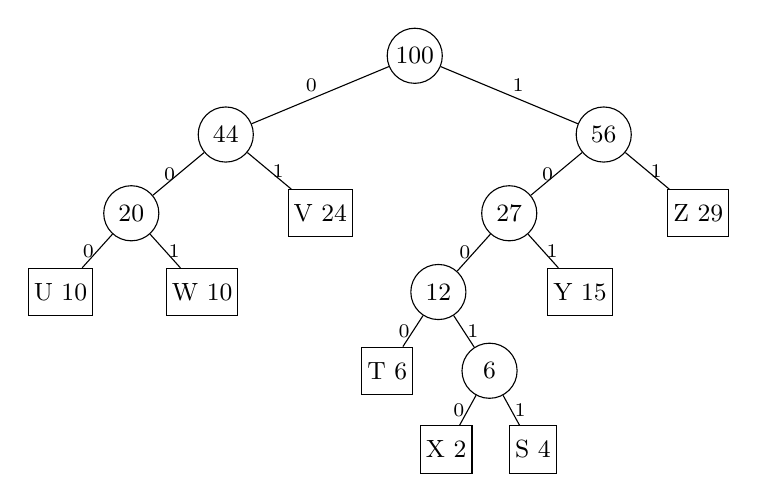
\begin{tikzpicture}[n/.style={circle,draw,inner sep=0pt,minimum size=7mm,font=\small},
  lf/.style={rectangle,draw,inner sep=2pt,minimum height=6mm,font=\small},
  e/.style={font=\scriptsize,midway,inner sep=1pt},
  level distance=10mm, level 1/.style={sibling distance=48mm}, level 2/.style={sibling distance=24mm},
  level 3/.style={sibling distance=18mm}, level 4/.style={sibling distance=13mm}, level 5/.style={sibling distance=11mm}]
\node[n] {100}
  child {node[n] {44}
    child {node[n] {20}
      child {node[lf] {U 10} edge from parent node[e,left] {0}}
      child {node[lf] {W 10} edge from parent node[e,right] {1}}
      edge from parent node[e,left] {0}}
    child {node[lf] {V 24} edge from parent node[e,right] {1}}
    edge from parent node[e,above left] {0}}
  child {node[n] {56}
    child {node[n] {27}
      child {node[n] {12}
        child {node[lf] {T 6} edge from parent node[e,left] {0}}
        child {node[n] {6}
          child {node[lf] {X 2} edge from parent node[e,left] {0}}
          child {node[lf] {S 4} edge from parent node[e,right] {1}}
          edge from parent node[e,right] {1}}
        edge from parent node[e,left] {0}}
      child {node[lf] {Y 15} edge from parent node[e,right] {1}}
      edge from parent node[e,left] {0}}
    child {node[lf] {Z 29} edge from parent node[e,right] {1}}
    edge from parent node[e,above right] {1}};
\end{tikzpicture}
\end{center}
霍夫曼碼與加權長度：
\begin{center}
\small
\begin{tabular}{c|cccccccc}
字母 & S & T & U & V & W & X & Y & Z \\
\hline
頻率 & 4 & 6 & 10 & 24 & 10 & 2 & 15 & 29 \\
編碼 & 10011 & 1000 & 000 & 01 & 001 & 10010 & 101 & 11 \\
長度 & 5 & 4 & 3 & 2 & 3 & 5 & 3 & 2 \\
頻率 $\times$ 長度 & 20 & 24 & 30 & 48 & 30 & 10 & 45 & 58 \\
\end{tabular}
\end{center}
總長 $20 + 24 + 30 + 48 + 30 + 10 + 45 + 58 = 265$，每個字母平均 $265 / 100 = 2.65$ 個位元。 檢查：總長也等於所有
合併得到的內部節點頻率之和，$6 + 12 + 20 + 27 + 44 + 56 + 100 = 265$，一致。 比㈠的編碼少了
$346 - 265 = 81$ 個位元（每百個字母），省下約 $23\%$。

步驟 2 有平手（T6 和合併出的 6），步驟 3 也有（U10 和 W10），左右標 $0$、$1$ 的方向也可以任選，所以霍夫曼碼不唯一；
但每一種選法得到的總長都是最小值 $265$（資結書定理~19.5），平均都是 $2.65$ 個位元。
\end{pastsoln}
